\documentclass[twocolumn,10pt]{jarticle}
\setlength{\columnsep}{3zw}
\usepackage{color}
\usepackage[dvipdfmx]{graphicx}
\usepackage{amsmath,amssymb}
\usepackage[linesnumbered,ruled,vlined]{algorithm2e}
\usepackage{bm}
\usepackage[top=10truemm,bottom=20truemm,left=15truemm,right=15truemm]{geometry}


% LaTeXについてはこちらを参考にして下さい.
% http://mikilab.doshisha.ac.jp/dia/seminar/latex/index.html

\title{中間発表}
\author{名前:松浦隆斗}
\date{日付: 8/13}

\begin{document}
\maketitle


\section{文献の引用}

%箇条書き
\begin{itemize}
      \item TeXでの参考文献の引用方法\cite{DE}.
      \item 複数の文献を引用する\cite{EA1,EA2}.
\end{itemize}



\section{数式の例}
各個体$\bm{x}_i$に対して,3個体$ \{  \bm{x}_{r1},\bm{x}_{r2},\bm{x}_{r3}  \} $を$\bm{x}_i$および互いに重複しないようにランダムに選択し,式
\eqref{eq:mutation}により変異ベクトル$\bm{v}_i$を生成する.

 \begin{eqnarray}
 \bm{v}_i= \bm{x}_{r1}+ F (\bm{x}_{r2}-\bm{x}_{r3})
\label{eq:mutation}
\end{eqnarray}

なお,子個体$\bm{u}_i$の要素$u_{i,j}$が探索空間 $\cal{S}$外に生成された場合,
以下の方法で修正を行う.
 \begin{eqnarray}
\begin{split}
u_{i,j} =
\left\{
\begin{array}{ll}
 2x^{L}_j-u_{i,j},  & \mbox{ $u_{i,j} <x^{L}_j $   } \\
  2x^{U}_j-u_{i,j},		   & \mbox{ $u_{i,j} >x^{U}_j $ } \\
\end{array}
\right.
\end{split}
\end{eqnarray}
ここで,$x^{L}_j, x^{U}_j (i = 1, 2, \dots ,D)$ は決定変数$x_j$の下
限値,上限値である.





\section{疑似コード}
変異ベクトル$\bm{v}_i$を親$\bm{x}_i$と交叉し,子個体$\bm{u}_{i}$を生成する.交叉はAlgorithm\ref{bin}のbinomial crossoverを用いる

\begin{algorithm}[htbp]
\DontPrintSemicolon
  
 $j_r=$select randomly from $[1,D]$;
 
  \For{$ j = 1$ \KwTo $D$} {
  
    \eIf{$ {\rm rand}(0,1) < CR$  {\rm or} $j=j_r  $}{
    $ u_{i,j}$=  $v_{i,j}$;
    }
    {
    $u_{i,j}$=  $x_{i,j}$;
    }
   }

\caption{binomial crossover}         
\label{bin}   
\end{algorithm}




\section{表および図の挿入}
実験で用いるモデルは,表\ref{tbl:MLP}に示すような2つの中間層を持つMLPとする.
また実験結果を,図\ref{fig:graph1}と図\ref{fig:graph2}に示す.

\begin{table}[htbp]
\begin{center}
\caption{表の説明}
\label{tbl:MLP}
\begin{tabular}{|l|c|c|}
\hline
Layer     & ユニット数 & 活性化関数  \\ \hline
中間層1 & hidden\_units1   & sigmoid関数   \\ \hline
中間層2 & hidden\_units2   & sigmoid関数      \\ \hline
出力層 & 3    & softmax関数        \\ \hline
\end{tabular}
\end{center}
\end{table}


\begin{figure}[htbp]
  \centering
  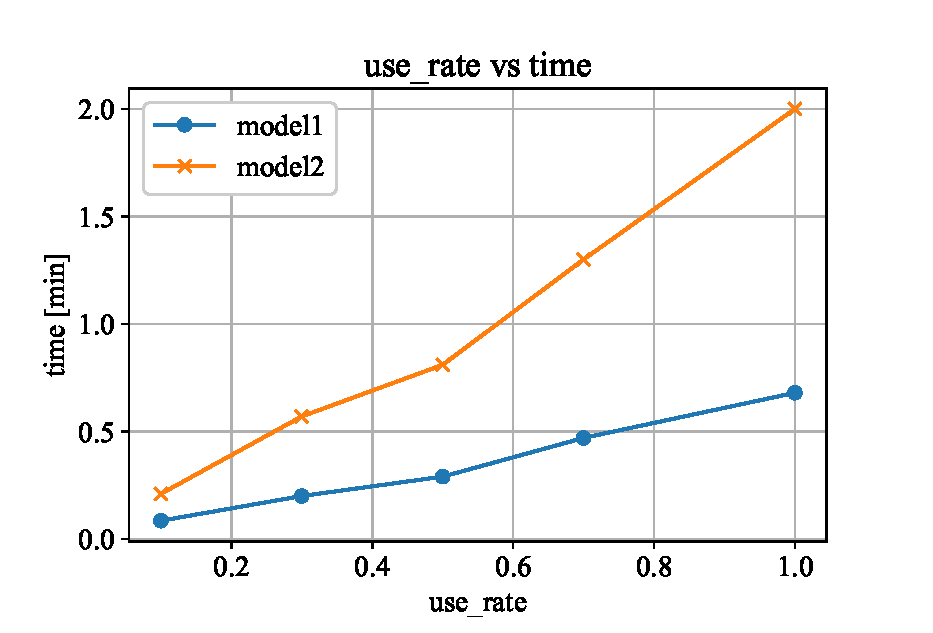
\includegraphics[width=.9\linewidth]{fig/graph1.eps}
  \caption{図の説明1}
  \label{fig:graph1}
\end{figure}

\begin{figure}[htbp]
  \centering
  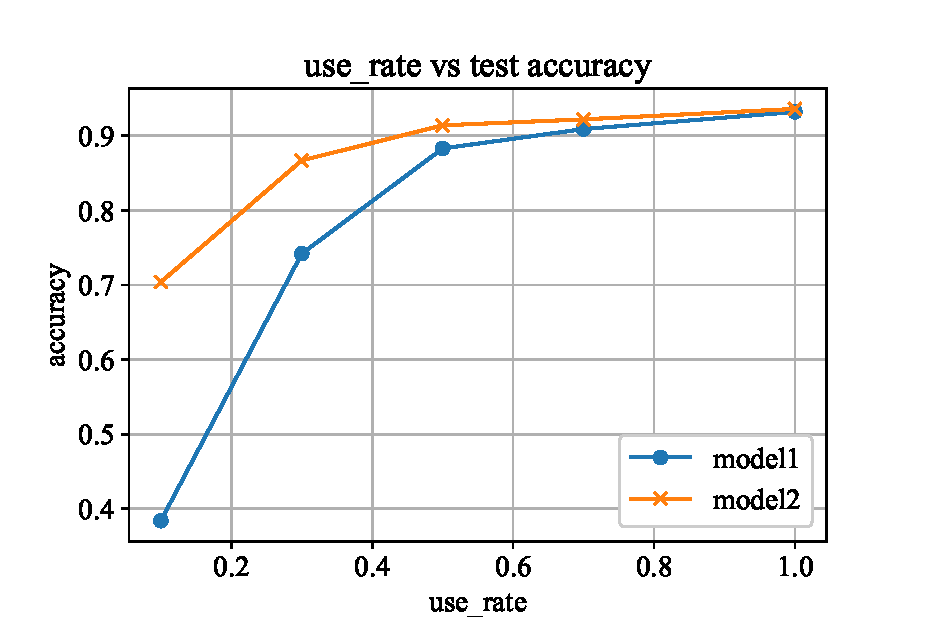
\includegraphics[width=.9\linewidth]{fig/graph2.eps}
  \caption{図の説明2}
\label{fig:graph2}
\end{figure}




\bibliography{btxsample}
\bibliographystyle{jplain}

%欧文用	和文用	特徴
%plain	jplain	参考文献をアルファベット順で出力する
%unsrt	junsrt	参考文献を引用された順で出力する


\end{document}